\appendix

\section{Similarity Transformations}

\begin{frame}[standout, plain, noframenumbering]
    Appendix

    % \medskip

    % \footnotesize
    % Sam Greydanus \quad Misko Dzamba \quad Jason Yosinski
\end{frame}

\begin{frame}
    \frametitle{Similarity Transformations -- Detailed}

    \begin{block}{Coordinate Isomorphism}
        Let $V$ be a vector space over $\mathbb{R}$ and $\mc{F} = \{f_1, \ldots,
        f_n \}$ be a basis of $V$.

        If $v \in V$, then $v = a_1f_1 + \cdots + a_n f_n$, where $a_i \in
        \mathbb{R}$ for $i = 1, \ldots, n$ are the \textit{coordinates} of $v$
        relative to $\mc{F}$. 
        
        The vector $a = \bmat{a_1 & \cdots & a_n}^\top \in
        \mathbb{R}^n$ is called the \textit{coordinate tuple} of $v$ relative to
        $\mc{F}$.

        The unique linear map $\varphi: \mathbb{R}^n \rightarrow V$ with
        $\varphi(e_j) = f_j$ for $j = 1, \ldots, n$ is called the
        \textbf{coordinate isomorphism} for $V$ and the basis $\mc{F}$. Here
        $e_j$ is the $j^{\textrm{th}}$ standard basis of $\mathbb{R}^n$.

        Thus $\varphi(a) = v$ if and only if $v = a_1 f_1 + \cdots + a_n f_n$.
    \end{block}
\end{frame}


\begin{frame}
    \frametitle{Similarity Transformations -- Detailed}

    \begin{block}{The matrix of a linear transformation}
        Let $T \in \End(V)$, i.e., $T: V \rightarrow V$ is a linear operator.
        
        The map $A = \varphi^{-1} \circ T \circ \varphi \in \End \mathbb{R}^n$
        and therefore has a matrix $[A]$; its $j^{\textrm{th}}$ column is
        $\varphi^{-1}(T(f_j))$ for $j = 1, \ldots, n$. This matrix is called the
        matrix of $T$ w.r.t. the basis $\mc{F}$.

        If $V \ni \tilde{v} = T(v)$ and $b$ and $a$ are the coordinate tuples of 
        $\tilde{v}$ and $v$, then $b = \varphi^{-1}\left(T(\varphi(a))\right) = 
        [A]a$. 

        Conversely, if $v \in V$ and $a = \varphi^{-1}(v)$ is the coordinate
        tuple of $v$ w.r.t. $\mc{F}$, and we set $b = [A]a$ and $\tilde{v} =
        \varphi(b)$, then $\tilde{v} = \varphi(A(a)) = T(v)$. That is $b = [A]a$ 
        if and only if $\tilde{v} = T(v)$.
    \end{block}
    
\end{frame}

\begin{frame}
    \frametitle{Similarity Transformations -- Detailed}

    \begin{block}{Theorem 1: Composition of linear transformations}
        Suppose $U$, $V$, and $W$ are vector spaces of finite dimension and a
        basis is chosen for each. 
        
        If $T \in \Hom(U, V)$ and $S \in Hom(V, W)$ with matrices $[A]$ and
        $[B]$, then the matrix of the linear transformation $S \circ T \in
        \Hom(U, W)$ w.r.t. the given bases is $[A][B]$.
    \end{block}
\end{frame}


\begin{frame}
    \frametitle{Similarity Transformations -- Detailed}

    Let $\mc{F} = \{f_1, \ldots, f_n \}$ and $\mc{F}^' = \{f_1^', \ldots,
    f_n^'\}$ be two bases for $V$. Let $\varphi$ and $\varphi^'$ be the
    coordinate isomorphisms, taking the standard basis in $\mathbb{R}^n$ to the
    first and second bases for $V$.

    Let $A = \varphi^{-1} \circ T \circ \varphi$, $B =
    {\left(\varphi^'\right)}^{-1} \circ T \circ {\varphi^'}$, $P = \varphi^{-1}
    \circ \varphi^'$ and $[P]$ be the matrix of $P: \mathbb{R}^n \rightarrow
    \mathbb{R}^n$. This means that element $(k,j)$, $p_{kj}$, of $[P]$ is found
    from 
    \vspace{-2mm}
    \small{
    \[ \varphi^{-1} \circ \varphi^' (e_j)  = \varphi^{-1}(f_j^') = 
     \varphi^{-1} \left( \sum_{k=1}^n p_{kj}f_k \right) = \sum_{k=1}^n p_{kj}e_k. \]}

    \vspace{-1mm}
    Similarly, the matrices $[A]$ and $[B]$ of $A$ and $B$ are found from 
    \footnotesize{
    \begin{align*}
        Ae_j &= \left( \varphi^{-1} \circ T \circ \varphi \right)e_j = 
        \varphi^{-1}\left( T(f_j) \right) = \varphi^{-1}\left( \sum_{k=1}^n 
        a_{ki}f_k \right) = \sum_{k=1}^n a_{ki} e_k. \\
        Be_j &= \left( \left(\varphi^'\right)^{-1} \circ T \circ \varphi \right)e_j = 
        \left( \varphi^'\right)^{-1}\left( T(f_j) \right) = 
        \left(\varphi^'\right)^{-1}\left( \sum_{k=1}^n b_{kj}f_k \right) = \sum_{k=1}^n b_{kj} e_k.
    \end{align*} 
    }
\end{frame}


\begin{frame}
    \frametitle{Similarity Transformations -- Detailed}

    We have
    \[ B = \left( \varphi^' \right)^{-1} \circ T \circ \varphi = \left(\varphi^'
    \right)^{-1} \circ \left(\varphi \circ A \circ \varphi^{-1}\right) \circ
    \varphi^' = P^{-1} \circ A \circ P. \]

    Now, Theorem 1 applies to yield \[ [B] = [P]^{-1} [A] [P], \] as desired.
    \hfill $\blacksquare$
\end{frame}


\begin{frame}
    \frametitle{Example 2.4 -- Revisited}

    \begin{table}
        \begin{tabular}{|c|c|c|}
            $V$ & $\mc{F}$ & $\mc{F}^'$ \\
            \hline
            $\mathbb{R}^3$ & $\left\{ x_0, y_0, z_0 \right\}$ & $\left\{ x_1,
            y_1, z_1 \right\}$
        \end{tabular}
    \end{table}

    Notice that, since $[P] = R_1^0$, we have \[ f_1^' = -f_3, \; \; f_2^' =
    f_2, \;\; f_3^' = f_1, \] i.e., \[ p_{31} = -1, \;\; p_{22} = 1, \;\; p_{13}
    = 1, \] and  
    $p_{ij} = 0$ for all other $i, j$. Furthermore, since $ A = \varphi^{-1}
    \circ T \circ \varphi$,

    \begin{table}
        \begin{tabular}{|c|c|c|c|}
            $\varphi$ & $\varphi^'$ & $\varphi^{-1} \circ \varphi^'$ & $[A]$ \\
            \hline
            $\id_{\mathbb{R}^3}$ & $P$ & $P$ & $R_{z,\theta}$
        \end{tabular}
    \end{table}

\end{frame}


\begin{frame}
    \frametitle{Example 2.4 -- Revisited}

    Let $v = 1 y_0 + 1 z_0 = -1 x_1 + y_1$. We compute,

    \vspace{-5mm}
    \[ A(v) = R_{z,\theta} \bmat{0 \\ 1 \\ 1} = \bmat{-s_\theta \\ c_\theta \\ 1}, \]
    \[
        B(v) = [P]^{-1}R_{z,\theta}[P] \bmat{-1 \\ 1 \\ 0} = 
        [P]^{-1}R_{z,\theta}\bmat{0 \\ 1 \\ 1} = [P]^{-1}\bmat{-s_\theta \\ c_\theta \\ 1} 
        = \bmat{-1 \\ c_\theta \\ -s_\theta}.
    \]

    \vspace{-5mm}
    \begin{figure}[bth]
        \centering
        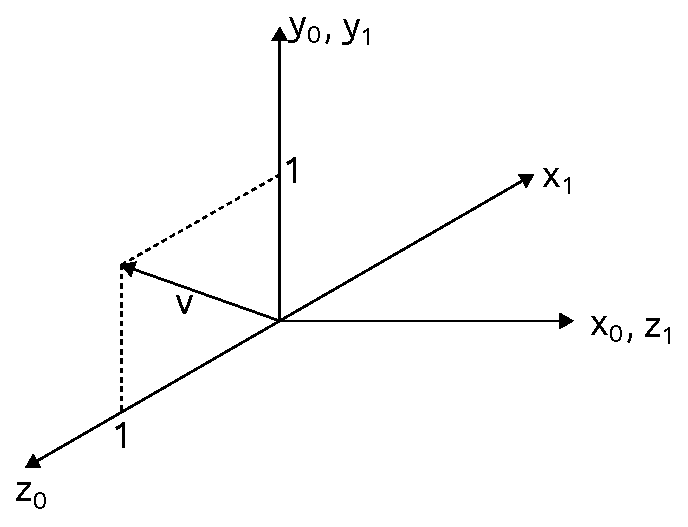
\includegraphics[width=0.5\textwidth]{figures/similarity_transform.eps}
        % \caption{\footnotesize }
    \end{figure}

\end{frame}

\begin{frame}
    \frametitle{Example 2.4 -- Revisited}

    Furthermore,
    \begin{align*}
      [B] = [P]^{-1}[A][P] &= \bmat{0 & 0 & -1 \\ 0 & 1 & 0 \\ 1 & 0 & 0}
      \bmat{c_\theta & -s_\theta & 0 \\ s_\theta & c_\theta & 0 \\ 0 & 0 & 1}
      \bmat{0 & 0 & 1 \\ 0 & 1 & 0 \\ -1 & 0 & 0} \\ &= 
      \bmat{1 & 0 & 0 \\ 0 & c_\theta & s_\theta \\ 0 & -s_\theta & c_\theta} = 
      R_{-x, \theta}.
    \end{align*}
\end{frame}